\documentclass[a4paper,11pt,twoside,openright]{book} % Type du document

% compiler avec : pdflatex, biber, makeglossaries, pdflatex, pdflatex


% +---------------------------------------------------------------+
% | Language and fonts
% +---------------------------------------------------------------+
\usepackage[T1]{fontenc}
\usepackage[utf8]{inputenc}
\usepackage[french]{babel}
\usepackage{lmodern}

% +---------------------------------------------------------------+
% | Paramètres
% +---------------------------------------------------------------+

\title{Création d'une cryptomonnaie écologique et confidentielle}
\author{Gil Balsiger}

% \newcommand{\TBtitle}{Création d'une cryptomonnaie écologique et confidentielle}
\newcommand{\TBsubtitle}{}%laisser vide si pas de sous-titre
\newcommand{\TByear}{2021}
\newcommand{\TBacademicYears}{2020-2021}

\newcommand{\TBdpt}{Département des Technologie de l'information et de la communication (TIC)}
\newcommand{\TBfiliere}{Filière Télécommunications}
\newcommand{\TBorient}{Orientation Sécurité de l'information}

% \newcommand{\TBauthor}{Gil Balsiger}
\newcommand{\TBsupervisor}{Prof. Alexandre Duc}
\newcommand{\TBindustryContact}{}
\newcommand{\TBindustryName}{}
\newcommand{\TBindustryAddress}{}



% TODO Résumé publiable

\newcommand{\TBresumePubliable}{
Dans ce travail... Ceci est le résumé publiable...
}

% +---------------------------------------------------------------+



% +-[set path]-------------------------------------+
\usepackage{template/TB-style}
\usepackage{template/TB-macros}
\usepackage{template/TB-template}
%\graphicspath{images/}

\makeglossaries
\newglossaryentry{bitcoin}
{
    name=Bitcoin,
    description={Cryptomonnaie inventée en 2008 par Satoshi Nakamoto}
}

\newglossaryentry{hash-function}
{
    name=fonction de hachage cryptographique,
    plural=fonctions de hachage cryptographiques,
    description={...}
}

\newglossaryentry{crypto-sym}
{
    name=cryptographie symétrique,
    description={...}
}

\newglossaryentry{crypto_asym}
{
    name=cryptographie asymétrique,
    description={...}
}

\newglossaryentry{vdf}
{
    name=verifiable delay function,
    description={...}
}

\newglossaryentry{signature}
{
    name=signature numérique,
    plural=signatures numériques,
    description={... \textit{Ne doit pas être confondue avec la signature électronique}}
}

\newglossaryentry{timestamp}
{
    name=réseau pair-à-pair,
    description={...}
}

\newacronym{prng}{PRNG}{Pseudo Random Number Generator}

\addbibresource{chapters/biblio.bib}

\begin{document}

\frontmatter
\pagestyle{empty}

% TITLE and template
% +---------------------------------------------------------------+

\TBmaketitle

\pagestyle{frontmatter}

\TBsecondTitle

\TBpreambule

\TBauthentification


% Cahier des charges
% +---------------------------------------------------------------+
\chapter{Cahier des charges}



\section*{Résumé du problème}

Le Bitcoin est la cryptomonnaie la plus connue et une des plus utilisées aujourd'hui en 2021. Cependant, elle n'est pas parfaite et certains points sur son fonctionnement et sa conception peuvent poser problème. Le premier est que la vérification des transactions est très consommatrice d'énergie. A titre d'exemple, la puissance totale de tous les mineurs de Bitcoin regroupés permettrait d'alimenter un pays de taille comparable aux Pays-Bas\cite{BTC_cons}. Le deuxième problème est que les transactions sont consultables publiquement ce qui pose un problème de confidentialité. Il est possible de voir le montant de chaque transaction et ainsi remonter la blockchain pour trouver le solde d'un compte. Cela n'est pas adapter à des transactions plus sensibles comme des versements de salaire par exemple.

\subsection*{Problématique}

En prenant en compte les deux problèmes majeurs du Bitcoin décrits ci-dessus, on peut en déduire que le Bitcoin n'est plus dans l'air du temps même si il est encore très populaire. La problématique est la suivante: il faut trouver une alternative écologique et confidentielle au Bitcoin.

\subsection*{Solutions existantes}

Aujourd'hui en 2021, il existe une multitude de blockchains et cryptomonnaies. Cependant la majorité d'entre elles utilisent le même principe énergivore que Bitcoin ou sont des tokens sur la blockchain Ethereum qui n'est, en 2021, ni plus écologique ni plus confidentielle que Bitcoin.

Mais il y a tout de même des solutions existantes. Il existe des algorithmes beaucoup moins énergivores que la vérification par preuve de travail (Proof-of-Work) utilisé par Bitcoin comme Proof-of-Stake ou encore Proof-of-Space. Concernant la confidentialité, il existes des blockchains confidentielles comme Monero ou Zcash. Cependant, il n'y a pas cryptomonnaie/blockchain qui utilise un algorithme écologie et confidentielle à la fois.

\subsection*{Solutions possibles}

Une solution possible pour résoudre cette problématique est de développer une blockchain qui utilisera un algorithme écologique pour vérifier les transactions comme du Proof-of-Stake ou du Proof-of-Space. Pour les raisons de confidentialité précédemment évoquées, les transactions devront être chiffrées au sein de la blockchain pour pas que leurs montants ou les adresses ne soient consultables publiquement.

\section*{Cahier des charges}

\subsection*{Objectifs}

\subsection*{Besoins}

\subsection*{Contraintes}

\subsection*{Déroulement}

\subsection*{Livrables}
Les délivrables seront les suivants :
\begin{enumerate}
\item Une documentation contenant :
	\begin{itemize}
	\item Une analyse de marché
	\item La décision qui découle de l’analyse
	\item Spécifications
	\item Les informations du module tel que le fonctionnement et les limitations 
	\item Une planification initiale et finale
	\item Un mode d’emploi
	\end{itemize}
\item Un module remplissant les objectifs défini au point 2.1.
\item Un software implémentant les améliorations s’il a été possible de les effectuer.
\end{enumerate}


% TOC
% +---------------------------------------------------------------+
\tableofcontents

\glsaddall % TODO: remove this line
\setglossarystyle{listhypergroup}
\printglossary


% Content
% +---------------------------------------------------------------+

\mainmatter
\pagestyle{plain}

\chapter{Introduction}
\label{ch:intro}


%exemple
\lipsum[1-4]



\chapter{Fonctionnement des cryptomonnaies}
\label{ch:presentation}

\section{Qu'est-ce qu'une cryptomonnaie ?}

Dans un premier temps, il est nécessaire de comprendre comment fonctionne une cryptomonnaie avant de pouvoir en créer une. Et il faut tout d'abord pouvoir définir \emph{qu'est-ce qu'une cryptomonnaie}.

Une cryptomonnaie est un ensemble de mécanismes cryptographiques utilisés dans le but de sécuriser un registre distribué afin d'obtenir un système de paiement décentralisé. Plus simplement, une cryptomonnaie est un système de paiement qui n'est pas régit par une entité centrale, comme une banque par exemple, et qui permet à tout le monde d'émettre des transactions qui seront incluses dans un registre. Ce registre est publique et partagé avec tous les utilisateurs via un réseau pair-à-pair. Le plus souvent, ce registre est représenté sous forme de chaîne de blocs, chaque bloc contenant ou un certain nombre de transactions. C'est la \emph{blockchain}.

Mais comme partout, il y a des personnes honnêtes mais aussi des gens malhonnêtes qui vont essayer d'abuser des failles du système. Dans le cas d'un système de paiement décentralisé, il n'y a pas de banque pour vérifier la validité des transactions ce qui pose un réel problème de sécurité. Du coup, pour rendre le système sûr, on utilise de la cryptographie. La cryptographie, grâce à des preuves mathématiques, rend la validité (ou non) des transactions irréfutable et permet à n'importe qui de vérifier les transactions stockées dans la blockchain.

Chaque utilisateur possède une copie de cette blockchain sur son ordinateurs, pour des raisons qui seront citées plus tard, et peut recevoir de nouvelles transactions d'autres utilisateurs et en envoyer lui-même. Voyons maintenant comment fonctionne plus en détails une blockchain avec une illustration simple et compréhensible dans la section suivante.

\section{La blockchain}

Comme vu ci-dessus, une cryptomonnaie est en fait un simple registre numérique dans lequel chacun peut ajouter des transactions. Imaginons maintenant un exemple simple avec les utilisateurs Alice, Bob et Charlie. Chacun d'entre eux peut ajouter une ligne au registre qui dit par exemple << Alice paie Bob 5 CHF >>, << Bob paie Charlie 8 CHF >>. Et, à interval régulier, ils se regroupent pour se transmettre l'argent qu'ils ont indiqué dans le registre.

\begin{figure}[H]
  \centering
  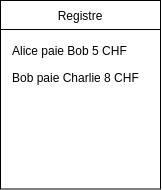
\includegraphics[width=4cm]{images/crypto_1.png}
  \caption{Exemple de registre de transactions}
\end{figure}

Seulement rien n'empêche Bob de rajouter la première ligne << Alice paie Bob 5 CHF >> autant de fois qu'il veut sans le consentement d'Alice.

\begin{figure}[H]
  \centering
  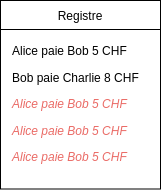
\includegraphics[width=4cm]{images/crypto_2.png}
  \caption{Bob inscrit de fausses transactions dans le registre}
\end{figure}

C'est là que la cryptographie rentre en jeu. Plus précisément les \glspl{signature}. Chaque transaction va être nécessairement accompagnée d'une signature. Les signatures numériques reposent sur de la \gls{crypto_asym}. C'est à dire que chaque utilisateur possède une pair de clé : une clé publique $pk$ et une clé privée (ou secrète) $sk$. La clé publique de chaque personne est partagée avec tous les autres utilisateurs du registre alors que la clé privée reste bien cachée chez son propriétaire et n'est jamais divulguée à qui que ce soit.

À la différence des signatures manuscrites sur papier qui sont à chaque fois presque identiques, une signature numérique change en fonction du message à signer. Pour signer un message, on utilise sa clé privée. On peut alors imaginer la signature d'un message $m$ avec la fonction suivante :

\begin{equation*}
  \mathsf{Sign}(m, sk) = \mathrm{signature}
\end{equation*}

Pour vérifier une signature numérique, on utilise la clé publique associée à la clé privée utilisée pour signer le message. Comme cette clé est connue de tous, tout le monde peut vérifier la signature du message de la manière suivante :

\begin{equation*}
  \mathsf{Verify}(m, \mathrm{signature}, pk) = \mathrm{\{Vrai, Faux\}}
\end{equation*}

Ainsi, au lieu de simplement ajouter une transaction au registre, les utilisateurs devront préalablement signer leur transaction et inscrire cette signature à coté de la transaction dans le registre. Cela permet de prouver que l'émetteur de la transaction est consentent. Les autres utilisateurs peuvent vérifier la signature de la transaction émise grâce à la clé publique de l'émetteur. Si la signature est correct, ils peuvent être quasiment certains que c'est bien l'émetteur de la transaction qui l'a signée car il est extrêmement difficile de forger une signature valide quand on ne possède pas la clé privée. 

Par exemple, si Alice souhaite inscrire une nouvelle transaction dans le registre, elle le ferait de la manière suivante :

\begin{align*}
  \mathrm{transaction_{Alice}} &= \textsf{"Alice paie Bob 5 CHF"}\\
  \mathrm{signature} &= \mathsf{Sign}(\mathrm{transaction_{Alice}, sk_{Alice}})
\end{align*}

\begin{figure}[H]
  \centering
  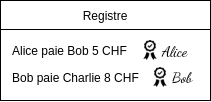
\includegraphics[width=6cm]{images/crypto_3.png}
  \caption{Les transactions du registre sont maintenant signées numériquement}
\end{figure}

De cette manière, Bob ne peut plus rajouter de lignes sans le consentement d'Alice car il ne possède pas sa clé privée. A noté également que lors de la vérification de la signature, la clé publique doit appartenir à la personne qui envoie de l'argent, sinon la transaction est rejetée. Cela fait sens car Bob peut signer << Alice paie Bob 10 CHF >> et la signature sera techniquement valide mais le contenu du message n'est pas juste. Bob ne peut pas demander de l'argent. C'est uniquement la personne qui signe la transaction qui donne de l'argent. 

Cependant, même si Bob ne connaît pas la clé privée d'Alice, il peut quand même ré-envoyer une ancienne transaction signée par Alice. Sa signature sera toujours valide.

\begin{figure}[H]
  \centering
  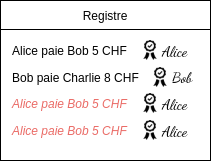
\includegraphics[width=6cm]{images/crypto_4.png}
  \caption{Bob inscrit deux anciennes transactions d'Alice}
\end{figure}

C'est pour cela qu'on inclut un identifiant unique, comme un nombre, à la transaction afin d'obtenir une signature différente à chaque transaction. Cela force Alice à refaire une signature à chaque nouvelle transaction et empêche Bob de réutiliser une ancienne signature valide d'Alice.

\begin{figure}[H]
  \centering
  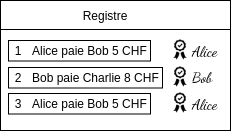
\includegraphics[width=6cm]{images/crypto_5.png}
  \caption{Un identifiant unique est signé avec la transaction}
\end{figure}

Maintenant, imaginons qu'un des utilisateurs, Charlie par exemple, doive beaucoup d'argent et ne vienne pas au rendez-vous pour payer les autres utilisateurs. Il peut écrire autant de transactions qu'il veut dans le registre et rien ne l'empêche de ne pas venir pour payer les autres. Il faut alors trouver un moyen où les utilisateurs n'ont pas besoin de se retrouver pour payer se qu'ils doivent.

On peut imaginer un système dans lequel les utilisateurs mettent une certaine somme d'argent dans un panier commun au début, disons 100 CHF et les premières lignes du registre indiquerait combien ils ont mis.

\begin{figure}[H]
  \centering
  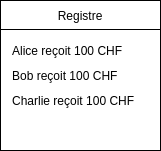
\includegraphics[width=4cm]{images/crypto_6.png}
  \caption{Premières lignes indiquant la somme initiale donnée par chaque utilisateur}
\end{figure}

Comme cela, on peut empêcher les utilisateurs de faire des transactions dont le montant dépasse ce qu'il possède dans le registre. Par exemple, si Charlie paie à Alice et Bob 50 CHF chacun, il ne pourra plus payer 10 CHF à nouveau à Bob car son solde sera trop faible.

\begin{figure}[H]
  \centering
  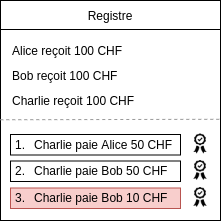
\includegraphics[width=5.5cm]{images/crypto_7.png}
  \caption{Charlie n'as pas assez d'argent pour effectuer la troisième transaction}
\end{figure}

Cela implique de conserver l'historique complet des transactions pour pouvoir donner le montant restant d'un utilisateur.

Avec ce système, on a une très bonne séparation entre l'argent dans le registre et l'argent réel. On peut même utiliser une monnaie propre au registre, par exemple des << jetons >>. Les utilisateurs sont libres d'échanger des jetons contre des francs suisse et inversément, cependant le taux de change entre les deux va dépendre de l'offre et de la demande puisqu'il y a un nombre limité de \emph{jetons} dans le registre. Par exemple, Alice peut donner à Bob 20 CHF et Bob, en échange, écrit une transaction dans le registre de 20 \emph{jetons} pour Alice.

Vient maintenant un autre problème avec ce registre. Qui est-ce qui gère le registre ? Qui est-ce qui vérifie si les transactions écrites sont valides ? Cela peut être une personne déléguée à cette tâche. C'est ce qui se fait souvent avec les cryptomonnaies privées car il est possible de désigner quelqu'un de confiance pour gérer le registre. Cependant, un des objectif de Satoshi Nakamoto lorsqu'il a écrit son document sur le Bitcoin est de faire un système de paiement \emph{décentralisé}. Un système dans lequel il n'y a pas d'entité centrale qui gère ce fameux registre. Ce qu'il propose est alors très simple: chaque utilisateur possède sa propre copie du registre. Comme ça c'est décentralisé et quand une personne souhaite effectuer une transaction, il l'envoie à tous les autres pour qu'ils l'ajoutent à leur registre. Mais on peut se demander: << Comment est-on sûr que tout le monde possède la même version du registre ? >>. Effectivement, si Bob envoie une transaction à Alice mais pas à Charlie, ils n'auront alors plus la même version du registre et par conséquent ne pourront plus calculer correctement leur solde lorsqu'ils voudront faire une nouvelle transaction. Du coup la question est : << À quelle version du register peut-on faire confiance ? >>.

Pour palier à ce problème, dans son papier, Satoshi Nakamoto explique qu'il faut avoir confiance dans le registre qui possède le plus de travail de calcul. Le \emph{travail de calcul} (computational work en anglais) utilise des \glspl{hash-function}. Une \emph{fonction de hachage} prend des données en entrée et donne une empreinte numérique en sortie. Cette empreinte semble complétement aléatoire mais n'est en réalité pas aléatoire car deux mêmes entrées donneront toujours la même empreinte. Une autre propriété importante des fonctions de hachage est le fait il est impossible de retrouver les données d'entrée à partie de l'empreinte. Il n'y a pas de meilleure méthode que de tester toutes les données possibles en entrée jusqu'à obtenir l'empreinte souhaitée. Et c'est sur cette propriété que se base l'algorithme de \hyperref[consensus:pow]{preuve de travail}.

Le \emph{consensus par preuve de travail} fonctionne de la manière suivante : on commence par découper le registre en blocs. Chaque bloc peut contenir un certain nombre de transactions. On assemble les données d'un bloc avec un nombre choisi et on passe le tout dans une fonction de hachage. On recalcul l'empreinte de ces données en modifiant le nombre jusqu'à que cette dernière commence par un nombre défini de \emph{zéros}. Plus l'empreinte commence par un nombre important de zéros plus le travail de calcul est grand. En effet, avec par exemple 30 << 0 >> au début de l'empreinte, en considérant que l'on hash un message aléatoire, la probabilité de trouver un hash commençant par 30 zéros est de $\frac{1}{2^{30}}$ soit 1 chance sur 1'073'741'824. Ce-dessous une illustration d'une preuve de travail :

\begin{figure}[H]
  \centering
  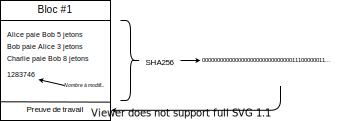
\includegraphics[width=\textwidth]{images/crypto_8}
  \caption{Calcul de la preuve de travail d'un bloc}
\end{figure}

Comme cela, un bloc n'est valide que lorsqu'il possède une preuve de travail correct, au même titre qu'une transaction n'est valide que lorsqu'elle est signée par l'envoyeur.

Pour créer une suite dans les blocs, on va inclure dans l'en-tête du bloc l'empreinte du bloc précédent. Ainsi, si on modifie les données d'un ancien bloc, cela changera son empreinte et il sera nécessaire de recalculer sa preuve de travail et celle de tous les blocs qui suivent.

\begin{figure}[H]
  \centering
  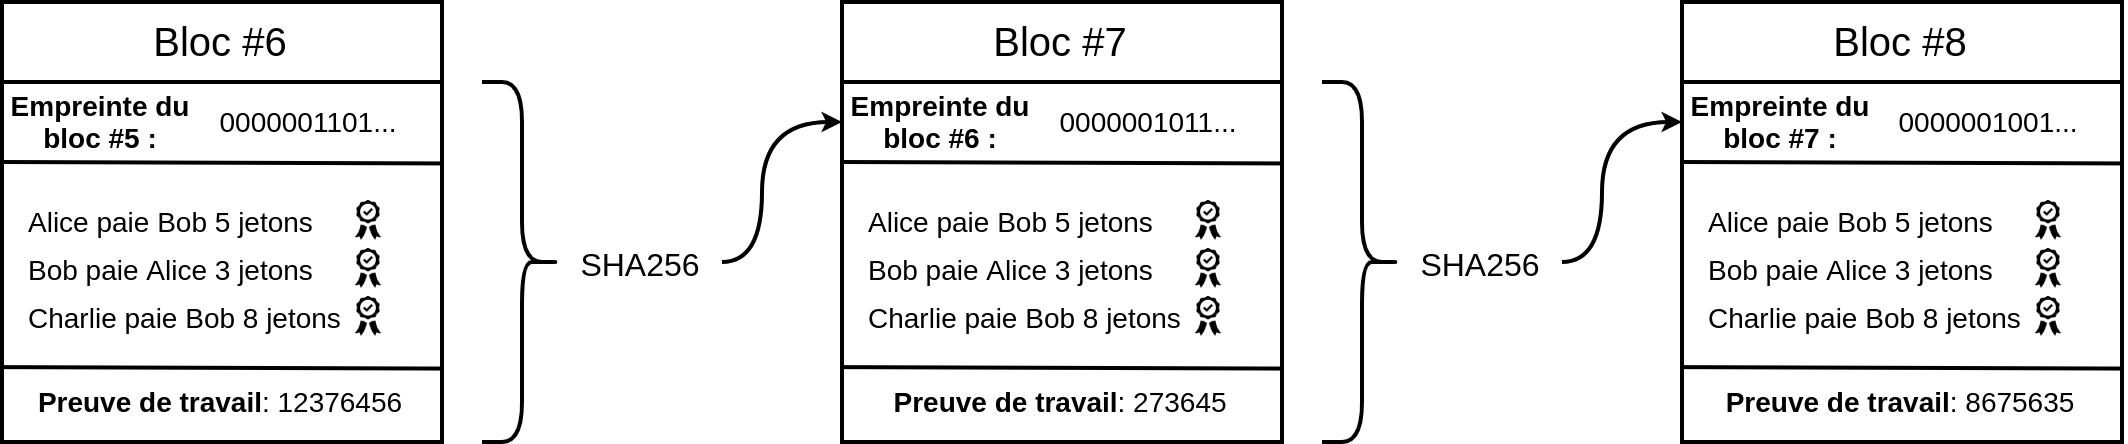
\includegraphics[width=\textwidth]{images/crypto_9}
  \caption{Chaîne de blocs}
\end{figure}

On a maintenant une chaîne de blocs, une << blockchain >>. Les utilisateurs vont, chacun de leur côté, essayer de faire un bloc en trouvant la preuve de travail associée. Le premier qui trouve une preuve de travail va publier le bloc. Les autres utilisateurs vont alors se baser sur ce nouveau bloc pour tenter de trouver la preuve de travail et publier leur bloc. C'est en quelques sortes une course à qui trouvera la preuve en premier et comme le travail de calcul dépend de la puissance de calcul des ordinateurs, les plus puissants auront plus de chance de la trouver en premier. 

Pour répondre à la question: << Comment être sûr que tout le monde à le même registre ? >>, il suffit de conserver la chaîne qui a le plus de travail de calcul. Dans la majorité des cas c'est la chaîne de blocs contenant le plus de blocs. Cela car en cas de fraude, l'attaquant devra être capable de trouver les preuves de travail tout seul plus rapidement que tous les autres utilisateurs. Par exemple, si Bob envoie un bloc avec des transactions de sa part à Alice mais ne l'envoie pas à Charlie, Alice aura une version frauduleuse de la chaîne. Pour qu'Alice continue à croire que c'est la bonne chaîne, Bob doit être capable de trouver la preuve de travail des nouveaux blocs avant Alice et Charlie qui cherchent également des preuves. Chose qui est difficile à faire car Bob ne possède qu'un ordinateur pour le calcul alors qu'Alice et Charlie ont chacun un ordinateur. Bob a du coup moins de puissance de calcul que les autres ce qui veut dire qu'Alice et Charlie, à eux deux, arriveront à terme à trouver des preuves plus rapidement que Bob. La chaîne frauduleuse de Bob ne sera alors plus la plus longue et Alice arrêtera de faire confiance à cette branche. Grâce à ce principe de preuve de travail, il est nécessaire de posséder plus de 50\% de la puissance de calcul total des utilisateurs pour pouvoir émettre une chaîne frauduleuse. C'est \emph{l'attaque des 51\%}. Ce principe a ailleurs été utilisé bien avant l'apparition des blockchains pour sécuriser des systèmes messageries contre les spams.

Nous avons vu ici l'illustration d'une blockchain simplifiée fonctionnant plus ou moins de la même manière que le Bitcoin avec quelques simplification. Avec Bitcoin, le nombre de zéros est défini par le réseau pour maintenir un temps de création de bloc d'environ 10 minutes. En effet, si on demande plus de zéros au début de l'empreinte, cela prendra plus de temps à calculer et inversément si on souhaite moins de zéros. Le réseau adapte alors ce nombre en fonction de la puissance disponible. Si des utilisateurs partent, il y aura moins de puissance de calcul disponible, le réseau diminuera alors le nombre de zeros et inversement si des utilisateurs se joigne au réseau.

On peut remarquer qu'une grande partie de la sécurité de la décentralisation repose sur le protocole de consensus et sur le fait que tous les utilisateurs soient d'accord sur la même version de blockchain. L'algorithme de consensus est en effet le cœur d'une blockchain et il en existe plein de différents, la preuve de travail (proof of work) étant le plus connu. C'est pour cela qu'un étude plus approfondie sur les protocoles de consensus est réalisée sur dans le chapitre suivant.


\chapter{État de l'art}
\label{ch:etat_art}

\section{Protocoles de consensus}

\textit{TODO: Petite intro de section}

\subsection{Proof of work}
\label{consensus:pow}

\textit{Proof of work} est un des tout premier protocole de consensus créé et est aujourd'hui un des plus utilisé. Il a au début été développé afin se prémunir des spams d'e-mail. Il a, en 2009, été adapté pour les blockchains par Satoshi Nakamoto en créant le \textbf{Bitcoin}.

Le protocole \textit{proof of work} utilise des ordinateurs appelés mineurs pour vérifier les blocs en résolvant des puzzles mathématiques. La résolution de ses puzzles requiert une grande puissance de calcule et une grande quantité d'énergie.

Techniquement, les mineurs utilisent des fonctions de hachage cryptographiques. Pour simplifier le processus, ces derniers doivent hacher l'ensemble des données du dernier bloc ($Bloc_n$) et un nombre ($p$) qu'ils peuvent choisir. Ce nombre est appelé la \textbf{preuve de travail}. Ci-dessous, un exemple du calcul réalisé par un mineur :

\begin{equation*}
    H = \textsf{SHA256}(\textsf{Bloc}_n \| p)
\end{equation*}

L'objectif est que le hash final $H$ commence par un certain nombre de 0. Ce nombre est fixé par le réseau. Comme les fonctions de hachage ne permettant pas de retrouver les données fournies en entrée à partir de la sortie, il n'y a pas d'autre moyen que de tester toutes les entrées possible jusqu'à ce que le hash commence par le bon nombre de 0. Ainsi le mineur va modifier la preuve de travail $p$ jusqu'à ce que le hash $H$ remplisse les conditions de la blockchain. 

Le nombre de 0 demandé en sortie est ce que l'on appelle la \textbf{difficulté} de la preuve de travail car plus il y a de 0 à la suite, plus il faudra de temps au mineur pour trouver la preuve de travail correspondante. Ce nombre de 0 est automatiquement définit par le réseau et est adapté à la puissance de calcul globale. C'est-à-dire que si la puissance augmente parce que de nouveaux mineurs ont rejoint le réseau, alors la difficulté augmentera également. Ceci afin de maintenir le temps de création d'un bloc à environ 10 minutes. Si des mineurs viendraient à quitter le réseau, il y aurait moins de puissance de calcul disponible, la difficulté sera alors revue à la baisse.

\subsection{Proof of stake, delegated proof of stake}
\label{consensus:pos}

Le protocole de \textit{proof of stake} (preuve d'enjeu en français) est le deuxième protocole le plus utilisé dans les blockchains actuelles. Il fonctionne sur un principe totalement différent que PoW car il ne requiert pas de puissance de calcul particulière ce qui en fait un bonne alternative en terme d'énergie. La cryptomonnaie Ether du réseau Ethereum est en train d'effectuer une migration vers du \textit{proof of stake} en 2021.

\textit{Proof of stake} fonctionnement sur le principe de staking. C'est-à-dire allouer une certaine quantité de cryptomonnaie au réseau. Cette monnaie bloquée appartient toujours à l'utilisateur mais ne peut plus être utilisée. Les nouveaux blocs seront créés par les utilisateurs qui mise le plus de jetons dans le réseau. Si ces personnes ne respectent pas leur engagement de contribuer au réseau de manière légitime, elle perdraient leur mise ce qui potentiellement ruinerait ces derniers. 

Avec cette architecture, pour pouvoir effectuer un acte de double dépense, il faudrait posséder et bloquer plus de la moitié de tous les jetons misés sur le réseau pour le contrôler ce qui rend ces attaques difficiles. Mais le fait que \textit{PoS} ne requiert pas de puissance de calcule amène d'autres problèmes qui n'existaient pas avec \textit{PoW} comme par exemple le problème du Nothing-to-stake.

Un autre problème que l'on peut remarquer avec ce protocole est que ce sont toujours les utilisateurs qui mise le plus qui sont prioritaires pour ajouter des blocs à la blockchain ce qui peut rendre le protocole trop centralisé alors que l'on recherche plutôt l'inverse.

Pour palier à ce problème, on a créé le \textit{delegated proof of stake}. Le principe est qu'on utilise cette fois-ci un système de vote dans lequel chaque utilisateur possède un nombre de voix proportionnel à la quantité de monnaie misée dans le réseau. Le système de vote varie en fonction des implémentations. Cela rend le protocole plus démocratique et ainsi ce ne sont pas toujours les mêmes entités qui ajoutent des blocs.

\subsection{Proof of authority, proof of reputation}
\label{consensus:poa}

\textit{Proof of authority} est un algorithme proposé par un des cofondateur d'Ethereum, Gavin Wood. Ce protocole se base lui sur la \textbf{réputation} des entités qui valident les blocs. A la différence du \hyperref[consensus:pos]{\textit{proof of stake}} qui se sert de la monnaie, \textit{PoA} met en valeur l'identité des validateurs qui sont sélectionnés comme entités de confiance.

Il y a ainsi un nombre limité de validateurs ce qui rend le réseau plus évolutif et efficace qu'un système avec du \hyperref[consensus:pow]{\textit{proof of work}} ou \hyperref[consensus:pos]{\textit{proof of stake}} car le consensus peut être atteint plus rapidement.

\textit{Proof of authority} est un protocole qui se porte particulièrement bien au \textbf{blockchains privées} permettant aux entreprise d'utiliser pleinement la technologie de la blockchain avec une architecture centralisée. En effet, l'aspect décentralisé du \hyperref[consensus:pow]{\textit{PoW}} et \hyperref[consensus:pos]{\textit{PoS}} peut ne pas convenir à certaines sociétés. D'un autre côté, ce protocole ne s'adapte pas très bien au blockchain publique du fait de sa centralisation. Centralisation que les utilisateurs des blockchains cherchent à évité pour des raisons de confidentialité (politique) et de sécurité (pannes, attaques).

On peut voir le \textit{PoA} comme un renoncement à la décentralisation dans un but d'efficacité mais ce mécanisme n'est pas vu de la même manière par tous. Notamment critiqué à cause des risques de corruption possibles si les identités des validateurs sont connus. En effet, un concurrent pourrait influencer les validateurs pour compromettre le réseau de l'intérieur.

En conclusion, \textit{PoA} est une bonne alternative au \hyperref[consensus:pow]{\textit{PoW}} et \hyperref[consensus:pos]{\textit{PoS}} pour les \textbf{blockchains privées} d'entreprise souhaitant utiliser ses technologies.

\subsection{Proof of space, proof of space-time}

\textit{Proof of space} est un protocole ressemblant à \hyperref[consensus:pow]{\textit{proof of work}} à la différence qu'au lieu de réaliser des puzzles mathématiques, les mineurs appelé farmers vont réalisés des preuves cryptographiques en allouant de l'\textbf{espace disque inutilisé} au réseau. Il est également appelé \textit{proof of capacity}. Ce principe permet de créer des preuves et valider les blocs rapidement avec un coût énergétique beaucoup plus faible que \hyperref[consensus:pow]{\textit{PoW}}. Ainsi on utilise la capacité de stockage comme ressource au lieu de la puissance de calcul.

Cependant, comme les vérifications peuvent être faites très rapidement comparé au Bitcoin où il faut trouver la solution au puzzle qui prend obligatoirement du temps, des nouvelle attaques apparaissent. Par exemple, un attaquant peut valider un grande quantité de blocs à la suite et les soumettre au réseau d'un seul coup. Chose qui n'est pas possible avec \textit{proof of work} puisque qu'il faut nécessairement trouver la preuve de travail avant de vérifier le suivant. Or trouver la preuve de travail prend du temps, beaucoup plus qu'avec \textit{PoSpace}. 

Pour éviter ce problème il existe plusieurs solutions. La première est de pénaliser les farmers agissant de manière malicieuse en intégrant un type de transaction propre aux pénalités. Cette manière de faire à été décrite dans le document de Spacemint \cite{DBLP:conf/fc/ParkKFGAP18}. Une autre solution est d'utiliser des preuve de temps (\textit{proof of time}) grâce à des fonctions à délai vérifiable (VDF). Cette solution à été choisie par le réseau Chia. Elle met en relation \textit{proof of space} et \textit{proof of time} pour donner un protocole de \textit{proof of space-time}. C'est-à-dire que les farmers prouvent au réseau qu'ils ont stocké un certaine quantité de données pendant un certain temps.

A noté que les données stockées sont inutiles dans le sens où elles ne représente rien de particulier. C'est donc le l'espace de stockage perdu au profit de la validation de blocs.

\subsection{Proof of replication, catalytic space}

\textit{Proof of replication} est une adaptation de \textit{proof of space} dans laquelle une majorité de l'espace de stockage peut être utilisé pour \textbf{stocker des données utiles}. Ici les farmers génèrent des preuves en prouvant qu'ils ont stocké des replicas de fichiers sur leurs disques. Ce principe est utilisé notamment dans la cryptomonnaie \href{https://filecoin.io/}{Filecoin}. En revanche, l'infrastructure à mettre en place avec un tel protocole est beaucoup plus complexe qu'avec du \textit{proof of space} simple.

\subsection{Proof of weight}

Le mécanisme de consensus par \textit{proof of weight} est un algorithme basé sur le modèle Algorand. Ce modèle basé sur un protocole de Byzantine agreement permet de vérifier rapidement les transactions et peut gérer beaucoup d'utilisateurs. 

Les blockchains utilisant \textit{proof of weight} assignent aux utilisateurs un \textbf{poids relatif} à une ressource qu'ils mettent à disposition de la blockchain. \textit{Proof of stake} est en quelque sorte un protocole de type \textit{proof of weight} dans lequel la quantité monnaie misée représente un poids. Plus ce poids est élevé, plus l'utilisateur à de chance de créer le prochain bloc.

Mais \textit{proof of weight} ne se limite pas à la quantité de monnaie misée sur le réseau comme \textit{proof of stake}. Par exemple, avec Filecoin, le poids est défini par la quantité de données IPFS d'un utilisateur. On peut également adapter un protocole de type \textit{proof of space} pour assigner aux utilisateurs un poids relatif à l'espace de stockage alloué au réseau.

\subsection{Proof of importance}

\textit{Proof of importance} est un algorithme qui met l'accent sur les utilisateurs les plus importants sur le réseau, c'est-à-dire les utilisateurs qui effectuent le plus de transactions. Ainsi, plus un utilisateur aura fait de transactions, plus il aura de chance d'être sélectionné pour créer le prochain bloc. Cela a pour but de favoriser le transfert et le mouvement de la monnaie à travers le réseau. En opposition avec \textit{proof of stake} qui favorise les utilisateurs à garder et bloquer leur argent.

\textit{Proof of importance} peut ainsi être utilisé en plus de proof of stake dans le but d'améliorer ce dernier. Cela résout une des principales critiques de \hyperref[consensus:pow]{\textit{PoW}} et \hyperref[consensus:pos]{\textit{PoS}} incite les utilisateurs à bloquer leur monnaie et se faisant centralise le système autour des personnes possédant le plus. \textit{PoI} en plus de \textit{PoS} permet d'éviter cette centralisation car les utilisateurs ne faisant pas de transaction seraient considéré comme moins important que les autres.

\subsection{Proof of burn}

\textit{Proof of burn} (preuve de destruction en français) est proposé comme une alternative à \textit{proof of work}. C'est un protocole qui permet aux utilisateurs de \textbf{brûler des coin} afin de prouver leur dévouement envers la blockchain. Ainsi plus un utilisateur brûle de coins, plus il aura de chance d'être sélectionné pour créer le prochain bloc. Ce principe utilise du coup moins d'énergie puisqu'il n'y a pas besoin de grande de puissance de calcul.

Le fonctionnement est le suivant: les utilisateurs souhaitant sécuriser le réseau vont envoyer des coins à une adresse d'incinération. Cette adresse rend les coins inutilisables ce qui crée une pénurie plus ou moins constante augmentant sa valeur potentielle. C'est un moyen d'investir dans la sécurité du réseau.

Il y a plusieurs moyen de mettre en oeuvre ce protocole. On peut sécuriser la blockchain en brûlant des Bitcoin ou bien certaines cryptomonnaie arrivent à le faire en brûlant leur propre monnaie.

En comparaison avec le \textit{proof of stake}, les coins sont ici brûlés et donc inutilisables après alors qu'avec la preuve d'enjeu, l'utilisateur souhaitant se retirer peut débloquer son argent et l'utiliser à nouveau. Cela ne crée ainsi pas de pénurie permanente.

Le \textit{proof of burn} a des avantages comme son aspect écologique ou encore le fait que les mineurs n'aient pas besoin de matériel particulier. Cependant il aussi des inconvénients comme le fait qu'il n'a jamais été mis en place à grande échelle. Le fait aussi de brûler des Bitcoin qui on été forgés avec du \hyperref[consensus:pow]{\textit{PoW}} rend le protocole tout de suite moins écologique.

\subsection{Proof of history}

\textit{Proof of history} \cite{proof:poh} est un protocole permettant de résoudre les problèmes de synchronisation au sein d'un système distribué grâce à des \textbf{fonctions à délai vérifiables (VDF)}. Ce n'est \textbf{pas} un protocole de consensus à lui seul cependant il est très intéressant et novateur c'est pourquoi il est inclu dans ce chapitre. Un des plus gros problème avec les blockchains et les systèmes décentralisés est la synchronisation des événements. S'assurer qu'un événement $B$ à bien eu lieu après un événement $A$ et avant un événement $C$ et qu'il est impossible d'en modifier l'ordre après coup. \textit{Proof of history} permet d'accomplir cela grâce à une fonction de délai vérifiable sous forme de fonction de hachage itérative. C'est une fonction qui permet de prouver qu'un certain temps réel s'est bien écoulé et est facilement vérifiable par d'autres utilisateurs.

Le protocole est ainsi une fonction de hachage qui s'appelle en boucle comme illustré dans le schéma ci-dessous.

\begin{figure}[H]
    \centering
    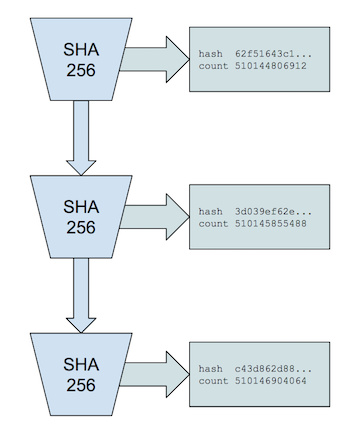
\includegraphics[width=8cm]{images/solana}
    \caption{Schéma simplifié de proof of history}
\end{figure}

On peut y injecter des entrées à tout moment. Cela va changer de manière imprédictible les données futures et ainsi ancrer les données dans l'historique de la chaîne de hachage.

Ce mécanisme a été inventé par Anatoly Yakovenko et est utilisé par la blockchain Solana. Ce protocole est utilisé avant un algorithme de consensus de type \emph{Delegated Byzantine Fault Tolerance}. L'auteur appelle le \emph{Proof of History}: \textbf{Clock before consensus}. C'est-à-dire que le \emph{PoH} ce charges de remettre dans l'ordre les événements avant faire le consensus.

Ce protocole permet d'obtenir une bande passante de transactions très élevée, jusqu'à 50'000 transactions par seconde d'après les créateurs rendant le protocole plus performant que Bitcoin qui atteint lui une douzaine de transactions par secondes.

% TODO: Réécrire Byzantine Fault Tolerance
\subsection{Byzantine Fault Tolerance}

\textit{Byzantine Fault Tolerance} est un large groupe de protocoles permettant d'atteindre un consensus entre les noeuds du réseau en prenant en compte le fait que des noeuds peuvent être indisponibles, transmettre des informations erronées ou être malhonnêtes. Il existe différents types d'algorithme basés sur \textit{BFT} mais la plus part d'entre eux ont un fonctionnement similaire. 

Avec les protocoles \textit{BFT}, pour simplifier, un noeud est choisi pour créer le prochain bloc. Cela peut se faire grâce à un système de vote ou aléatoirement sans tenir compte d'une ressource en particulier. Le bloc est ensuite transmis à travers le réseau à plusieurs autres noeuds. Ces autres noeuds vont faire certaines vérifications et transmettre le bloc à leur tour et le consensus est atteint lorsque la majorité des noeuds a reçu le bloc et est d'accord sur la version de la chaîne de bloc. Ensuite un autre noeud est sélectionné pour le bloc suivant.

Il est facile simple de détecter les fraudes car si les blocs sont invalides ils seront supprimés par les autres noeuds. Cependant les protocoles \textit{BFT} sont pour la plupart vulnérables aux \textbf{attaques de Sybil} donc si une majorité des noeuds du réseau sont malhonnêtes, il sera impossible d'obtenir un consensus correct. C'est pour cela qu'ils sont souvent associer à d'autres protocoles comme \hyperref[consensus:pow]{\textit{PoW}} ou \hyperref[consensus:pos]{\textit{PoS}}.

\section{Analyse des protocoles}

Tous ces protocoles permettent d'une manière ou d'une autre de sécuriser la blockchain. Cependant ils ne respectent pas tous les contraintes écologiques de ce travail. Afin de pouvoir faire un choix, ces protocoles seront ci-dessous analysés afin de pouvoir trouver les mieux adaptés selon différents critères comme l'impact écologique, la facilité d'implémentation, les ressources disponibles et autre points importants.

\begin{itemize}
    \item \textbf{Proof of work}: ce protocole est certes le plus populaire et possède le plus de ressources sur internet, il est cependant le moins écologique de tous. C'est principalement pour cette raison qu'il ne sera pas question d'implémenter un protocole comme \textit{PoW} ou autres protocoles basés sur ce dernier. A noté que l'implémentation d'un algorithme de \textit{proof of work} est plus simple que la majeur partie des autres protocoles.
    \item \textbf{Proof of stake}: écologiquement plus intéressant que PoW, la preuve d'enjeu peut se trouver être une bonne alternative en terme de consommation d'énergie. Cependant, comme elle fonctionne sur le principe de bloquer de l'argent pour la sécurité du réseau, cela implique qu'il faut nécessairement un certaine quantité d'argent dès le début, ce qui est problématique pour commencer une blockchain à partir de rien. \textit{Ethereum} qui effectue une migration de PoW vers PoS possède déjà beaucoup d'argent en circulation pouvant être bloqué pour faire de la preuve d'enjeu convenablement. Mais à partir de rien, c'est conceptuellement difficile ce qui rend l'implémentation plus compliquée.
    \item \textbf{Proof of authority}: PoA est une bonne alternative pour les blockchains privées. Son implémentation est plutôt simple car il n'y a pas besoin d'utiliser des ressources particulières comme de la puissance de calcul, une somme d'argent ou de l'espace de stockage. Il suffit de simplement vérifier les noeuds validateurs qui sont explicitement autorisés par une entité. Il est du coup difficile pour n'importe qui de devenir validateur et contribuer à la sécurité du réseau. C'est pourquoi elle est adaptée à des blockchains privées or, dans ce travail, on souhaite implémenter une cryptomonnaie publique où tout le monde peut contribuer.
    \item \textbf{Proof of space}: ce protocole est intéressant du point de vue énergétique car il fonctionne comme \textit{PoW} mais ne demande pas de puissance de calcule mais de l'espace de stockage à la place. Son empreinte écologique est du coup beaucoup plus faible. Son implémentation est cependant plus complexe car il faut utiliser des graphs permettant de prouver qu'un utilisateur à bien stocker tant de données et ces dernier ne sont pas forcément facile à réaliser. Mais il existe des implémentations de \textit{proof of space} comme Chia ou encore Spacemesh ce qui fournissent déjà un quantité de ressources acceptable. Ce protocole est un très bon candidat pour ce travail car bien adapté.
    \item \textbf{Proof of replication}: ce protocole possède les mêmes avantages que proof of space vue juste au dessus mais avec en plus l'avantage que les données stockées sont des données utiles. Mais en revanche l'implémentation est beaucoup plus compliquée. Prouver qu'un utilisateur à stocker des réplicas de fichiers est plus complexe mathématiquement que de prouver qu'il a stocker des données pseudo-aléatoires. Il y a des ressources comme Filecoin qui sont disponibles et peuvent aider à comprendre le fonctionnement mais cela reste trop de travail pour ce projet.
    \item \textbf{Proof of weight}: étant une famille de protocole, il n'existe pas un protocole mais plusieurs avec par exemple \textit{proof of stake} qui peut être associé à du \textit{proof of weight} d'une certaine manière. En tant que tel, \textit{proof of weight} est assez jeune et très peu utilisé avec peu d'information disponible sur internet, c'est pourquoi il sera mis de côté mais reste un protocole intéressant sachant qu'on peut dériver du \textit{PoSpace} en \textit{PoWeight} en assignant un poids relatif à l'espace de stockage.
    \item \textbf{Proof of importance}: le principe de ce protocole est également intéressant mais est, à nouveau, très jeune avec peu de ressources disponibles. Se lancer dans l'implémentation d'un tel protocole est trop risqué.
    \item \textbf{Proof of burn}: \textit{Proof of burn} a un concept assez spécial et peut être un protocole écologique si les coins brûlé sont les coins de la cryptomonnaie même. Cependant ce protocole n'a jamais été testé à large échelle et se trouve être assez théorique avec très peu d'implémentations existantes et de ressources disponibles le rendant peu attractif.
    \item \textbf{Proof of history}: probablement le protocole le plus intéressant avec \textit{proof of space} car c'est également un protocole plus écologique que \textit{PoW}. Son concept est innovant et utilisé dans la blockchain Solana donc déjà plus ou moins déployé. Cependant les concepts utilisés sont plus obscures que ceux utilisés avec \textit{proof of space} ce qui rend son implémentation plus compliquée car plus difficile à comprendre. Il y a quelques ressources disponible sur la documentation de Solana mais moins que sur le réseau Chia par exemple.
    \item \textbf{Byzantine Fault Tolerance}: cette famille de protocole englobe tous les algorithmes de consensus vu ci-dessus, ce n'est pas un protocole à proprement dit. On utilise un ou plusieurs protocoles vu précédemment pour avoir de la \textit{Byzantine Fault Tolerance} au sein d'un réseau d'ordinateurs distribués. Cela pour éviter principalement les attaques de Sybil.
\end{itemize}

% TODO: Attaque sur les blockchains
\section{Attaques sur les blockchains}

\subsection{Attaque Sybil}

\dots

\subsection{Attaque des 51\%}

\dots

\subsection{Grinding attacks}

\dots

\subsection{Reécriture de l'historique}

\dots

\subsection{Problème du "Nothing-to-stake"}

\dots

\section{Mécanismes de sécurisation}

La technologie de la blockchain apporté par Bitcoin est révolutionnaire. Pouvoir faire des paiements sans passer par un organisme centrale est génial mais le problème pour réaliser cela est qu'il faut conserver publiquement un registre de toutes les transactions. Les entrées et sorties des transactions sont identifiées par des adresses dérivées des clés publiques des utilisateurs. Les transactions sont ainsi pseudonymes. Satoshi Nakamoto l'a dit dans son whitepaper: \textit{The public can see that someone is sending an amount to someone else, but without information linking the transaction to anyone.}

Mais les transaction ne sont pas anonymes. On peut quand même voir le montant, de qui et vers qui va l'argent même si on ne sais pas forcément qui sont derrières les adresses. Il faut bien faire la distinction entre \emph{anonyme} et \emph{pseudonyme}.

Cependant, il existe des blockchains qui permettent d'anonymiser leurs transactions. Rendant illisible le montant et les adresses ainsi que tout autres données. Les deux cryptomonnaies les plus connue à ce sujet sont présentées ci-dessous. 

\subsection{Zcash}

\dots

\subsection{Monero}

\dots

\section{Cryptomonnaies de 3ème génération}

On peut qualifier le Bitcoin de 1ère génération de cryptomonnaie. Il y a eu ensuite Ethereum et l'apparition des smart-contracts considéré comme cryptomonnaie de 2ème génération. Et maintenant il y a les cryptomonnaies de 3ème génération qui tentent de résoudre les problèmes présents avec le Bicoin et Ethereum. Notamment les soucis de performance et de stockage.

\subsection{Performance des blockchains}

Un point important est la performance des blockchains. Or le Bitcoin ne peut traiter que 4 à 5 transactions par seconde ce qui le rend très peu performant comparé au réseau VISA qui traite environ 2000 transactions par seconde en moyenne et peu monter plus haut en cas de forte affluence. Le problème vient du fait qu'il faut 10 minutes pour générer un bloc et que chaque bloc fait au maximum 1 mégaoctet. Ces informations sont codées en dur dans le code source de Bitcoin ce qui veut dire qu'il est possible de les modifier pour améliorer les performances du réseau Bitcoin. Mais alors pourquoi les développeurs ne l'ont pas fait ? 

Il y a deux possibilités: 1. réduire le temps de génération d'un bloc et 2. augmenter la taille maximum d'un bloc. 

La première possibilité est compliquée à mettre en place car la propagation d'un nouveau bloc à travers le réseau prend du temps. Réduire le temps de création implique de réduire la difficulté de la preuve de travail ce qui fera que plus de mineurs généreront plus de blocs rendant le consensus plus compliqué à cause du nombre de mineurs présent sur le réseau et d'un propagation lente.

La deuxième possibilité à fait de grands débats au sein de la communauté. C'est facile d'augmenter la taille des blocs mais cela implique que la blockchain prendra plus d'espace de stockage à l'avenir. Certains développeurs étaient pour une augmentation et d'autres non ce qui est venu à créer \emph{Bitcoin Cash}, un "hard fork" de Bitcoin. Les développeurs de Bitcoin Cash ont décidé d'augmenter la taille maximum des blocs. Ils ont choisi un bloc dans la blockchain Bitcoin et ont créé une nouvelles branches à partir depuis laquelle les nouveaux blocs de Bitcoin Cash seront créés. Par ailleurs, si vous aviez des Bitcoins avant la séparation vous avez du coup le même montant en Bitcoin Cash (BCH) mais aussi en Bitcoin. Comme les deux branches sont séparées l'une de l'autre, c'est comme si les coins s'étaient dupliqués.

\subsection{Cardano}

% TODO: Écrire Cardano
\dots

\subsection{IOTA}

% TODO: Écrire IOTA
\dots

\subsection{Solana}

% TODO: Écrire Solana
\dots

\documentclass[../tb_report.tex]{subfiles}

\begin{document}

\chapter{Proof of space}
\label{ch:pospace}

\section{Introduction}

La \emph{preuve d'espace} (ou \emph{proof of space} en anglais) est un algorithme de consensus similaire à la preuve de travail à la différence qu'au lieu d'effectuer des calculs de manière continue pour trouver une preuve satisfaisant les conditions de la difficulté de la blockchain, les mineurs appelés farmers avec \emph{PoSpace} vont trouver des preuves à partir d'un challenge grâce à une certaine quantité de données allouées sur le disque dur. 

Il existe principalement deux constructions pour faire du proof of space : une basée sur le compromis temps-mémoire de Hellman \cite{DBLP:conf/asiacrypt/AbusalahACKPR17} et une basée sur des \emph{hard-to-pebble graphs} \cite{DBLP:conf/crypto/DziembowskiFKP15}.

Pour ce travail, il a fallu faire un choix d'un algorithme à implémenter. Ce choix c'est porté sur la construction des compromis temps-mémoire car il y plus de ressources disponibles. De plus, la construction des graphs de type \emph{hard-to-pebble} s'avère être trop compliquée pour un travail comme celui-ci, c'est aussi pourquoi elle a été écartée.

Ce chapitre explique le fonctionnement général du protocole principalement tiré de la blockchain Chia. Les détails d'implémentation sont décrits dans le chapitre suivant [\ref{ch:realisation}].

\section{Résumé du protocole}

Dans un premier temps, les données sont générées par le farmer dans une étape appelée \textbf{plotting}. Ce sont des données pseudo-aléatoires qui ne représentent rien de particulier. D'autres algorithmes pour stocker des données utiles existent comme \emph{proof of catalytic space} ou \emph{proof of replication} utilisés dans la blockchain \href{https://filecoin.io/}{Filecoin} par exemple.

En suite, un farmer peut prouver qu'il a bien les données qu'il dit avoir stockées en trouvant une ou plusieurs preuves répondant à un challenge donné. C'est l'étape du \textbf{farming}.

Lors de la \textbf{vérification}, le vérificateur récupère la prevue est à partir de celle-ci, recalcule le challenge et vérifie s'il correspond à celui envoyé précédemment.

Ainsi, on peut considérer \emph{proof of space} comme est un protocole dans lequel nous avons :

\begin{enumerate}
  \item un vérificateur qui envoie un challenge à un farmer et
  \item un farmer qui peut prouver au vérificateur qu'il a bien alloué la quantité d'espace spécifiée à un instant $t$.
\end{enumerate}

\begin{figure}[H]
  \centering
  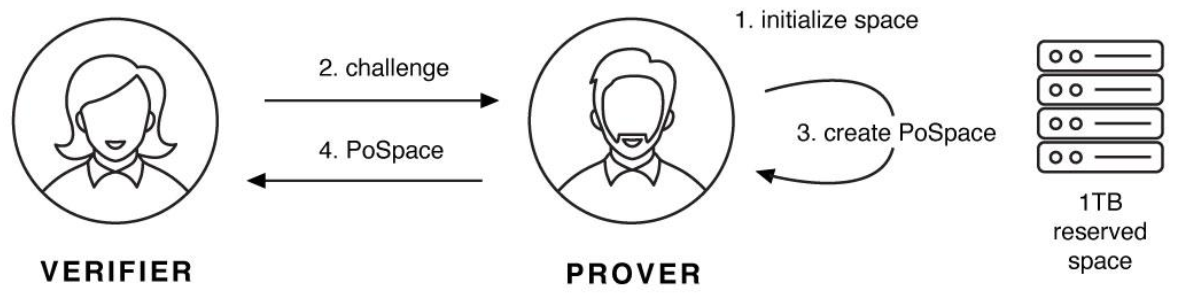
\includegraphics[width=\textwidth]{images/pospace.png}
  \caption{Diagramme du protocole \emph{proof of space} montrant les différentes étapes. Tiré de \cite{chia:consensus}}
\end{figure}

\section{Plotting}

Le plotting est un procédé non-interactif dans le lequel le farmer va créer les données qui seront stockées et qui permettront de trouver les preuves d'espace liées aux challenges. Ce procédé peut être long, cela peut prendre de plusieurs heures à plusieurs jours suivant la quantité de données allouées.

La construction de cette preuve d'espace est basée sur la construction de Chia \cite{chia:construction}, elle-même basée sur les compromis temps-mémoire \emph{Beyond Hellman} \cite{DBLP:conf/asiacrypt/AbusalahACKPR17}. Elle a cependant été simplifiée pour pouvoir être réalisée dans le temps imparti de ce travail. 

Le principe

Le farmer choisi un nombre $k$ pour définir combien il souhaite allouer d'espace. La quantité de données finale est exponentielle par rapport à ce nombre $k$. Le processus générera un plot dont la taille sera environ égale à $780 \times k \times 2^{k-10}$ \cite{chia:consensus}. Le temps de la génération dépend de la puissance de l'ordinateur effectuant le plotting puisqu'il s'agit principalement d'exécution de fonctions de hachage. C'est le CPU qui sera beaucoup solicité durant cette étape. Le contenu du plot sera 4 tables de données pseudo-aléatoires. Chaque table contiendra $2^k$ entrées et chaque entrée d'une table $i$ pointra vers 2 entrées dans la table précédente ($i-1$). La première table quant à elle contientra ce qu'on appelle les \emph{x-values}. Ce sont simplement des nombres entiers de $0$ à $2^k-1$. Ainsi. une preuve d'espace correspond à 8 \emph{x-values} ($2^{\textsf{nombre de table} - 1} = 2^3 = 8$). A noter que ce processus à besoin de plus d'espace de stockage qu'indiqué au début car il générera des données qui seront ensuite nettoyées et compressées mais la génération des tables occupera plus de place que la taille finale du plot. C'est important à prendre en considération car pour un plot final de 1 To, il faudra par exemple 1.5 To de libre pour la génération. 





Les détails de l'implémentation et des choix réalisés sont décrits dans le chapitre suivant.

\section{Farming}

\dots

\section{Vérification}

\dots

\section{Sécurité et attaques}

\dots

\end{document}

\chapter{Dossier de réalisation}
\label{ch:realisation}

%exemple
\lipsum[1-4]


\chapter{Conclusion}

\section{Résultat final}

Ce travail a mis l'accent tout particulièrement sur l'analyse des protocoles de consensus et l'implémentation du \emph{proof of space}. Et c'est dans un deuxième temps, après avoir réalisé une implémentation fonctionnelle du proof of space que la création d'une blockchain a été entreprise. La blockchain développée avait pour objectif de donner un exemple d'utilisation du proof of space avec un cas concret. De plus, sa confection m'a permis d'en savoir plus sur le fonctionnement des cryptomonnaies.

Concernant les protocoles de consensus, il y en a beaucoup qui sont intéressants mais nouveaux et donc n'ont pas énormément été utilisé concrètement. Côté écologie, le proof of work est le pire loin devant les autres mais reste avec la preuve de sécurité la plus fiable. Mais le soucis écologique qu'il pose tend les blockchains à migrer vers d'autres protocoles plus efficaces et consommant moins d'énergie. Le proof of space est un protocole tout à fait intéressant qui a suscité pas mal d'intérêt. C'est pourquoi il été choisi pour être implémenté. Le proof of stake est peut-être le deuxième protocole le plus populaire après le proof of work, il est cependant plus difficile à mettre en place sur une nouvelle cryptomonnaie puisque qu'il faut justement miser une partie de cette monnaie. Il reste quand même un bon protocole écologique.

Il est difficile de faire un classement des protocoles étudiés mais on peut dire que proof of space et proof of stake sont deux protocoles répondant aux problèmes écologiques dû au faible besoin de puissance de calcul. Proof of authority sera plus adapté pour des blockchains privées puisqu'il est plus facile de mettre en place des validateurs de confiance dans le secteur privé. Proof of history n'est certes pas un protocole de consensus, il peut s'intégré à un protocole pour permettre un synchronisation rapide comme proof of stake avec la blockchain Solana.

Étant donnée l'importance placée sur le proof of space, c'est concernant ce dernier qu'il y a le plus de résultats. Notamment au niveau des performances où plusieurs tests de benchmark on été réalisé. La conclusion de l'implémentation est qu'il est possible de créer un plot dans le but de trouver des preuves pour un challenge donné. La construction est basée sur la phase 1 du protocole de Chia \cite{chia:construction} et a été finalement entièrement implémentée (la phase 1 pas les autres). La génération du plot final se fait en temps exponentiel par rapport à une constante $k$ alors que la vérification de preuves est très efficace et réalisable en temps constant.

\section{Difficultés rencontrées}

La majeur partie des difficultés rencontrées concerne l'implémentation du proof of space. C'était une construction assez difficile à comprendre au début et il a fallu du temps pour pouvoir l'implémenter. Il a fallu apprendre à utiliser des librairies pour manipuler des bits, ce dont on a pas forcément l'habitude. On travaille le plus souvent en octet. Il a fallu trouver un moyen d'améliorer les performances avec \emph{Rayon}, une librairie de multithreading, pour obtenir un temps d'exécution convenable. Et enfin il a fallu réaliser un moyen de trier les données sur le disque. Parce que comme le protocole génère beaucoup de données, tout ne peut pas être conservé en mémoire, il faut les stocker sur le disque dur. Après la génération, les tables doivent être triées avant de pouvoir générer la suivante. Comme ces tables peuvent atteindre plusieurs giga-octets, il a fallu développer un algorithme de tri externe. C'était une des partie les plus compliquées à faire.

Mais dans l'ensemble il n'y a pas eu de difficulté trop importante qui ait pu bloquer l'avancée du projet. Il a fallu apprendre et comprendre rapidement et il a fallu écrire pas mal de code.


\section{Objectifs non-réalisés}

Mise à part tout le travail réalisé sur le proof of space et la blockchain, il y a quand même des objectifs qui n'ont pas été atteint. Notamment le souhait de créer une cryptomonnaie confidentielle. Cet aspect précis n'as pas été réalisé par manque de temps, l'implémentation du proof of space ayant pris bien 60\% du travail. Il aurait fallu analyser les blockchains \emph{Monero} et \emph{Zcash} pour connaître quelles méthodes étaient utilisées pour sécuriser les transactions et voir s'il est possible d'en ajouter une à notre blockchain. Malheureusement cette partie du travail n'a pas pu être faite.

\section{Améliorations possibles du projet}

Il y a une infinité d'améliorations possibles pour le projet mais voici une petite liste non-exhaustive d'améliorations :

\begin{itemize}
  \item Rendre les transactions confidentielles (comme Zcash ou Monero)
  \item Implémenter les phases suivantes du proof of space (nettoyage et compression)
  \item Ajouter un moyen d'avoir un consensus sécurisé (avec des VDF par exemple)
\end{itemize}

\section{Conclusion personnelle}

Venant d'une proposition personnelle, ce travail était très important pour moi et je suis content d'avoir pu le faire comme travail de Bachelor. Il m'a permis d'en apprendre beaucoup plus sur les cryptomonnaies sur le côté technique, ce que je souhaitais initialement en proposant ce sujet. Il m'a aussi permis de découvrir des protocoles de consensus particuliers notamment le proof of space dont j'ai particulièrement apprécier implémenter la construction. J'aurai évidemment souhaiter avoir plus de temps pour pouvoir améliorer ma blockchain, peut-être faire la partie mise en réseau ou bien la confidentialité des transactions mais je suis déjà très content d'avoir pu délivrer une blockchain fonctionnelle intégrant un protocole de proof of space.

% +---------------------------------------------------------------+
\cleardoublepage
\addcontentsline{toc}{chapter}{Bibliographie}
\nocite{*}
\printbibliography

\listoffigures
\listoftables

% Annexes
% +---------------------------------------------------------------+
\appendix

\input{chapters/appendix}

\end{document}
